
%===================================================
\chapter{The User Entry Operation}
\label{sec:UserEntry}
%===================================================

\begin{traceunit}{FD.External.TISUserEntryOp}
\traceto{FS.External.TISUserEntryOp}
\end{traceunit}

\label{sec:userEntry}
This operation is a multi-stage operation and will be presented as 
a number of operations with preconditions on the internal $state$.
The state transition diagram for user authentication and entry is
given in Figure \ref{fig:userEntry}. Before user authentication and
entry the system is in the $quiescent$ state, on completion of the
user authentication and entry the system will return the to
$quiescent$ state.

\begin{figure}[htbp]
  \begin{center}
    \leavevmode
    \resizebox{\textwidth}{!}{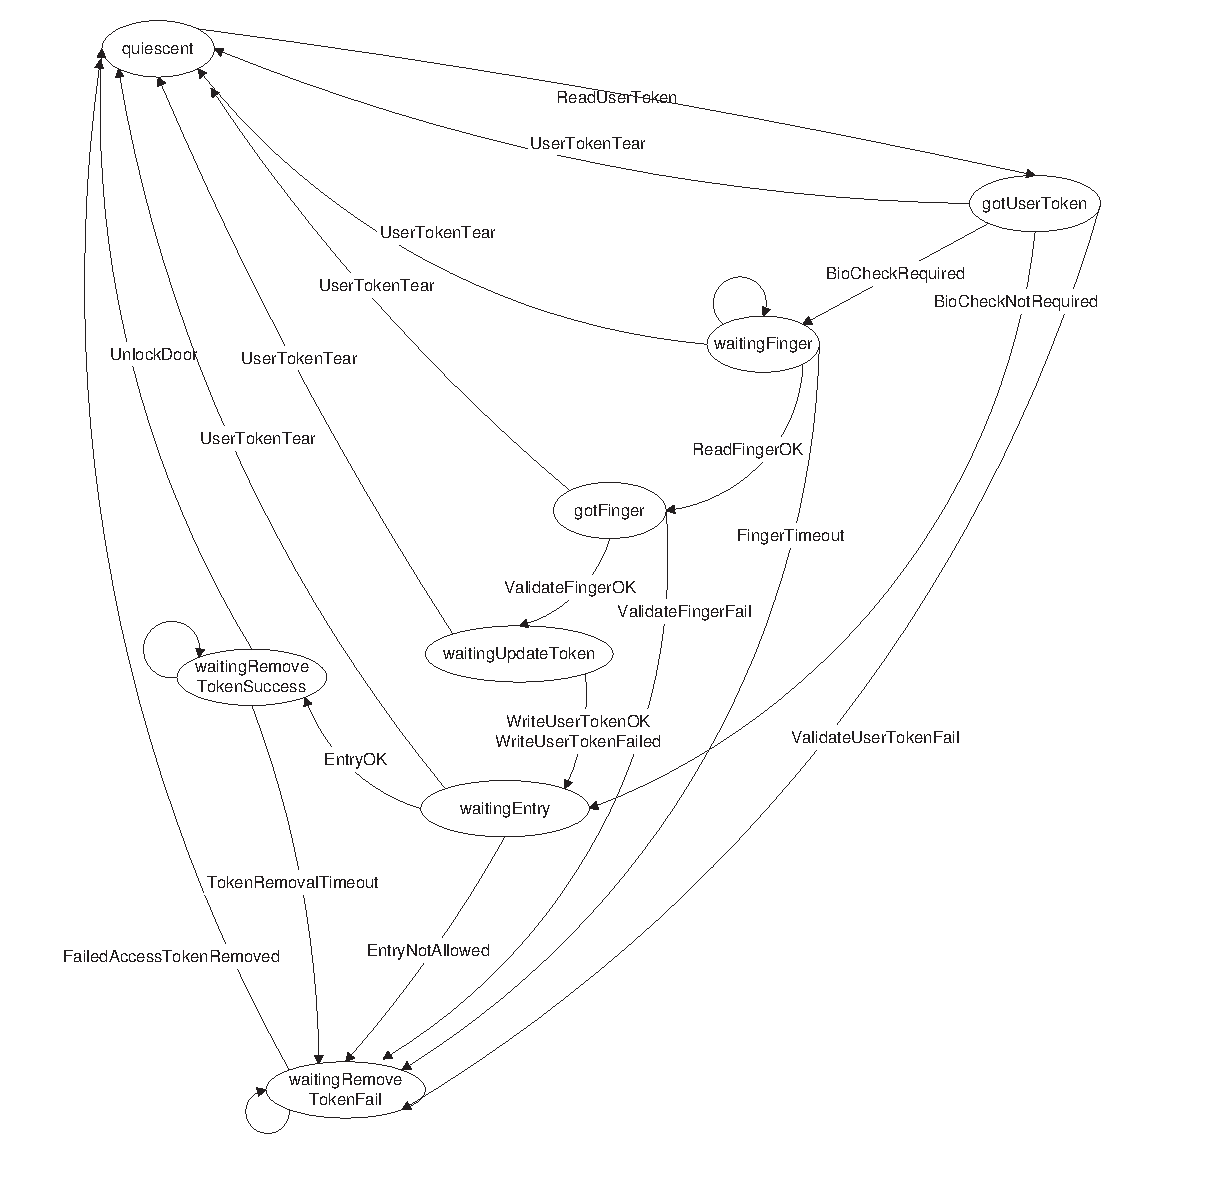
\includegraphics{50_1_entry.eps}}
    \caption{User Authentication and Entry state transitions}
    \label{fig:userEntry}
  \end{center}
\end{figure}

The process of user authentication and entry follows the following
stages:

\begin{itemize}
\item

Before any user attempts access, the system is $quiescent$.
\item
Once the token has been inserted and the information read off,
the status moves to $gotUserToken$, waiting for the system to validate
the token. 
\item
Once the token has been successfully validated the 
status moves to $waitingFinger$,
waiting for the user to give a fingerprint.
\item
Once the fingerprint has been read, the status moves to $gotFinger$,
waiting for the system to validate the fingerprint.
\item
Once a fingerprint has been successfully validated,
the status moves to $waitingUpdateToken$,
waiting to write the Auth Cert to the token.
\item
Once the Auth Cert has been written, the status moves to
$waitingEntry$, where it determines whether the role has
current entry privileges.
\item
If the role has current entry privileges the status moves to
$waitingTokenRemoveSuccess$, where the system system waits for 
the token to be removed.
\item
Once the token has been removed
the latch will be unlocked if the role has current access privileges
to the enclave and the ID Station will return to $quiescent$.
\end{itemize}
In the case of a failure in the user validation process the status
moves to  $waitingRemoveTokenFail$, waiting until the token has been removed before returning to a
$quiescent$ state.

This specification separates opening the door from having a valid Auth
Certificate. It is possible for a role to be entitled to enter the
enclave but not use the workstations (for example such clearence might
be given to a buildings maintenance engineer). TIS
configurations will ensure that having a valid Auth Certificate will
guarantee that entry to the enclave is permitted. 

\begin{traceunit}{FD.Enclave.ResetScreenMessage}
{FS.Enclave.ResetScreenMessage}
\end{traceunit}

The message displayed on the screen will indicate that the
system is busy while a user entry is in progress that blocks
administrator activity. Once the user entry activity becomes
non-blocking then an appropriate message is displayed on the screen.

\begin{schema}{ResetScreenMessageC}
        \Delta InternalC
\\      \Delta AdminC
\\      currentScreenC, currentScreenC' : ScreenC
\where
        UserEntryInProgress'
 \land currentScreenC'.screenMsgC = busyC
\\      \lor
\\      \lnot UserEntryInProgress' 
\\ \t1 \land (enclaveStatusC' = enclaveQuiescent \land rolePresentC' = \Nil 
\\ \t3          \land currentScreenC'.screenMsgC = welcomeAdminC
\\ \t2 \lor enclaveStatusC' = enclaveQuiescent \land rolePresentC' \neq \Nil 
\\ \t3          \land currentScreenC'.screenMsgC = requestAdminOpC
\\ \t2 \lor enclaveStatusC' = waitingRemoveAdminTokenFail 
\\ \t3          \land currentScreenC'.screenMsgC = removeAdminTokenC
\\ \t2 \lor enclaveStatusC' \notin 
        \{ enclaveQuiescent, waitingRemoveAdminTokenFail \} 
\\ \t3          \land currentScreenC'.screenMsgC = currentScreenC.screenMsgC)
\end{schema}

The user entry operation leaves much of the $IDStation$ state
unchanged. The context of this operation is summarised:

\begin{schema}{UserEntryContextC}
        \Delta IDStationC
\\      RealWorldChangesC
\also
        \Xi ConfigC
\\      \Xi AdminTokenC
\\      \Xi KeyStoreC
\\      \Xi AdminC
\\      \Xi KeyboardC
\\      \Xi FloppyC
\\      AddElementsToLogC
\\      LogChangeC
\\      ResetScreenMessageC
\also
      \Xi TISControlledRealWorldC
\where
        enclaveStatusC' = enclaveStatusC
\\      statusC \neq waitingEntry \implies tokenRemovalTimeoutC' = tokenRemovalTimeoutC
\\      statusC' \neq waitingFinger \implies fingerTimeout' = fingerTimeout
\also
        auditTypes~ newElements? \subseteq USER\_ENTRY\_ELEMENTS \cup USER\_INDEPENDENT\_ELEMENTS
\end{schema} 

\begin{Zcomment}
\item
The following state components may change $UserTokenC$, $InternalC$
$DoorLatchAlarmC$, $CertificateStore$, $StatsC$ and $AuditLogC$.
\item
The components of the real world controlled by TIS remain unchanged.
\item
The $tokenRemovalTimeoutC$ is only updated if the current status is
$waitingEntry$.
\item
The $fingerTimeout$ may only be updated if the current status becomes
$waitingFinger$.
\item
All elements logged during user entry operations either relate to the
user entry or are independent of any operation.
\item
Changes are logged and $newElements?$ will be added to the Audit Log.
\end{Zcomment}

Each of the following sub-operations is performed within the above context.

%----------------------------------------------------------------------
\section{User Token Tears}
%----------------------------------------------------------------------
\begin{traceunit}{FD.UserEntry.UserTokenTorn}
\traceto{FS.UserEntry.UserTokenTorn}
\end{traceunit}

During the operation the user may tear his token from the reader
prematurely. There are a number of internal states during which token
removal is deamed erroneous.

If the user tears the Token out before the operation is complete then
the operation is terminated unsuccessfully.

\begin{schema}{UserTokenTornC}
        UserEntryContextC
\also
	ClearUserToken
\\      \Xi DoorLatchAlarmC
\\      AddFailedEntryToStatsC      
\\      \Xi CertificateStore
\where
        UserHasDeparted
\\      statusC \in \{ gotUserToken, waitingUpdateToken,
waitingFinger, gotFinger, waitingEntry \}
\also
        currentDisplayC' = welcome
\\      statusC' = quiescent 
\also
        auditTypes~ newElements? \cap USER\_ENTRY\_ELEMENTS = 
        \{ userTokenRemovedElement \} 
\also
        \exists_1 element : AuditC @ element \in newElements? 
\\ \t1  \land element.elementId = userTokenRemovedElement
\\ \t1  \land element.logTime \in nowC \upto nowC'
\\ \t1  \land element.user = extractUser~ currentUserTokenC
\\ \t1  \land element.severity = warning
\\ \t1  \land element.description = noDescription

\end{schema}
\begin{Zcomment}
\item
The $userTokenRemovedElement$ is the audit entry recording that the
token has been removed from the reader outside the enclave. 
\end{Zcomment}

%-------------------------------------------------------------------
\section{Reading the User Token}
%-------------------------------------------------------------------
\begin{traceunit}{FD.UserEntry.TISReadUserToken}
\traceto{FS.UserEntry.TISReadUserToken}
\end{traceunit}


The User Entry operation is initiated when TIS is in a $quiescent$ state
and detects the presence of
a token in the user token reader (which resides outside the enclave). 

A user entry operation may start while the $enclaveStatus$ is
quiescent ($enclaveQuiescent$) or the enclave is waiting for a failed
admin token to be removed.

When the user token is first detected as present, its presence is
audited and the internal status changes. It is not until the token has 
been validated that we can be sure of the user's identity, however the
token ATR should provide a token ID which can be used as the user identity.

No other aspects of the system are modified.

\begin{schema}{GetPresentUserTokenC}
        UserEntryContextC
\also
        ReadUserTokenC
\\	\Xi DoorLatchAlarmC
\\      \Xi StatsC
\\      \Xi CertificateStore
\where
        UserEntryCanStart
\also
        userTokenPresenceC' = userTokenPresenceC
\\      currentUserTokenC' = userTokenC
\also
	currentDisplayC' = wait
\\	statusC' = gotUserToken

\also
        auditTypes~ newElements? \cap USER\_ENTRY\_ELEMENTS = 
        \{ userTokenPresentElement \} 
\also
        \exists_1 element : AuditC @ element \in newElements? 
\\ \t1  \land element.elementId = userTokenPresentElement
\\ \t1  \land element.logTime \in nowC \upto nowC'
\\ \t1  \land element.user = extractUser~ currentUserTokenC'
\\ \t1  \land element.severity = information
\\ \t1  \land element.description = noDescription

\end{schema}

The operation to read the user token is as follows:

\begin{zed}
        TISReadUserTokenC \defs GetPresentUserTokenC \hide ( newElements? )
\end{zed}


%--------------------------------------------------------------------
\section{Validating the User Token}
%--------------------------------------------------------------------
Once TIS has read a user token it must validate the contents of that
token.

A user token is valid for entry without biometric checks if the token
contains a consistent authorisation certificate which is current.

A user token is valid for entry into the enclave if the token is
consistent, current and the ID
certificate, Privilege certificate and I\&A certificate can be validated.

\begin{traceunit}{FD.UserEntry.BioCheckNotRequired}
\traceto{FS.UserEntry.BioCheckNotRequired}
\end{traceunit}

In the case where there is a
valid Authorisation certificate the biometric checks are bypassed.

\begin{schema}{BioCheckNotRequiredC}
        UserEntryContextC
\also
        \Xi UserTokenC
\\      \Xi DoorLatchAlarmC        
\\      \Xi StatsC
\\      \Xi CertificateStore
\where
        \lnot UserHasDeparted
\\      statusC = gotUserToken
\also
        UserTokenWithOKAuthCertC
\also
        statusC' = waitingEntry
\\      currentDisplayC' = wait
\also
        auditTypes~ newElements? \cap USER\_ENTRY\_ELEMENTS = 
        \{ authCertValidElement \} 
\also
        \exists_1 element : AuditC @ element \in newElements? 
\\ \t1  \land element.elementId = authCertValidElement
\\ \t1  \land element.logTime \in nowC \upto nowC'
\\ \t1  \land element.user = extractUser~ currentUserTokenC
\\ \t1  \land element.severity = information
\\ \t1  \land element.description = noDescription
\end{schema}

\begin{traceunit}{FD.UserEntry.BioCheckRequired}
\traceto{FS.UserEntry.BioCheckRequired}
\traceto{FDP\_RIP.2.1}
\end{traceunit}


The biometric checks are only required if the Authorisation
Certificate is not present or not valid. In this case the remaining
certificates on the card must be checked.

An audit element is logged indicating that the authorisation
certificate is not valid.
The audit element will reference a user, the owner of the token, there is
no additional information in the description. 

\begin{schema}{BioCheckRequiredC}
        UserEntryContextC
\also
        FlushFingerDataC
\\      \Xi UserTokenC
\\      \Xi DoorLatchAlarmC        
\\      \Xi StatsC
\\      \Xi CertificateStore
\where
        \lnot UserHasDeparted
\\      statusC = gotUserToken
\also
        \lnot UserTokenWithOKAuthCertC \land UserTokenOKC
\also
	currentDisplayC' = insertFinger
\\	statusC' = waitingFinger
\\      fingerTimeout' = currentTimeC + fingerWaitDuration
\also
        auditTypes~ newElements? \cap USER\_ENTRY\_ELEMENTS = 
        \{ authCertInvalidElement \} 
\also
        \exists_1 element : AuditC @ element \in newElements? 
\\ \t1  \land element.elementId = authCertInvalidElement
\\ \t1  \land element.logTime \in nowC \upto nowC'
\\ \t1  \land element.user = extractUser~ currentUserTokenC
\\ \t1  \land element.severity = information
\\ \t1  \land element.description = noDescription
\end{schema}

\begin{traceunit}{FD.UserEntry.ValidateUserTokenFail}
\traceto{FS.UserEntry.ValidateUserTokenFail}
\end{traceunit}

If the token cannot be validated then this is logged and the user is
required to remove the token. The audit element detailing this failure
will contain the user if this can be extracted from the token. The
description will indicate the point of failure of the card.

\begin{schema}{ValidateUserTokenFailC}
        UserEntryContextC
\also
        \Xi UserTokenC
\\      \Xi DoorLatchAlarmC        
\\      \Xi StatsC
\\      \Xi CertificateStore
\where
        \lnot UserHasDeparted
\\      statusC = gotUserToken
\also
        \lnot UserTokenOKC \land \lnot UserTokenWithOKAuthCertC
\also
	currentDisplayC' = removeToken
\\      statusC' = waitingRemoveTokenFail
\also
        auditTypes~ newElements? \cap USER\_ENTRY\_ELEMENTS = 
        \{ userTokenInvalidElement \} 
\also
        \exists_1 element : AuditC; description! : TEXT @ 
\\ \t1  element \in newElements? 
\\ \t1  \land element.elementId = userTokenInvalidElement
\\ \t1  \land element.logTime \in nowC \upto nowC'
\\ \t1  \land element.user = extractUser~ currentUserTokenC
\\ \t1  \land element.severity = warning
\\ \t1  \land (element.description = description! \land UserTokenNotOK)

\end{schema}
\begin{Zcomment}
\item
$UserTokenNotOK$ defines the error description.
\end{Zcomment}

%...............................
\subsection{Determining whether biometric checks are required}
%...............................


\begin{zed}
        DetermineBioCheckRequired \defs (BioCheckRequiredC \lor
        BioCheckNotRequiredC) \hide (newElements? )
\end{zed}

There are lots of things that may go wrong with validation of the user
token. In each case the system will terminate the operation unsuccessfully.

\begin{zed}
        TISValidateUserTokenC \defs 
                (BioCheckRequiredC 
                \lor BioCheckNotRequiredC
                \lor ValidateUserTokenFailC 
\\ \t4 \lor
        [~UserTokenTornC | statusC = gotUserToken ] ) \hide (newElements? )
\end{zed}

%-----------------------------------------------------------------
\section{Reading a fingerprint}
%----------------------------------------------------------------

\begin{traceunit}{FD.UserEntry.ReadFingerOK}
\traceto{FS.UserEntry.ReadFingerOK}
\end{traceunit}


A finger will be read if the system is currently waiting for it (has
not waited too long) and
the user Token is in place.

\begin{schema}{ReadFingerOKC}
        UserEntryContextC
\also
        \Xi DoorLatchAlarmC
\\	\Xi UserTokenC
\\      \Xi StatsC
\where
        \lnot UserHasDeparted
\\	statusC = waitingFinger
\\	fingerPresenceC = present
\\      currentTimeC \leq fingerTimeout 
\also
\\	currentDisplayC' = wait
\\	statusC' = gotFinger
\also
        auditTypes~ newElements? \cap USER\_ENTRY\_ELEMENTS = 
        \{ fingerDetectedElement \} 
\also
        \exists_1 element : AuditC @ element \in newElements? 
\\ \t1  \land element.elementId = fingerDetectedElement
\\ \t1  \land element.logTime \in nowC \upto nowC'
\\ \t1  \land element.user = extractUser~ currentUserTokenC
\\ \t1  \land element.severity = information
\\ \t1  \land element.description = noDescription
\end{schema}


\begin{traceunit}{FD.UserEntry.NoFinger}
\traceto{FS.UserEntry.NoFinger}
\end{traceunit}


If there is no finger present then, if we have not allowed sufficient
attempts to get and validate a finger, nothing happens. 

\begin{schema}{NoFingerC}
        \Xi IDStationC
\\      RealWorldChangesC
\also
        UserEntryContextC
\\      \Xi TISControlledRealWorldC
\where
        \lnot UserHasDeparted
\\      statusC = waitingFinger
\\      currentTimeC \leq fingerTimeout 
\\      fingerPresenceC = absent
\end{schema}

\begin{traceunit}{FD.UserEntry.FingerTimeout}
\traceto{FS.UserEntry.FingerTimeout}
\end{traceunit}

Alternatively, TIS may have tried to obtain a valid finger for too
long, in which case the user is requested to remove the token and 
the operation is terminated unsuccessfully. 


\begin{schema}{FingerTimeoutC}
        UserEntryContextC
\also
        \Xi UserTokenC
\\      \Xi DoorLatchAlarmC
\\      \Xi StatsC       
\where
        \lnot UserHasDeparted
\\        statusC = waitingFinger
\\      currentTimeC > fingerTimeout
\also
        currentDisplayC' = removeToken
\\      statusC' = waitingRemoveTokenFail
\also
        auditTypes~ newElements? \cap USER\_ENTRY\_ELEMENTS = 
        \{ fingerTimeoutElement \} 
\also
        \exists_1 element : AuditC @ element \in newElements? 
\\ \t1  \land element.elementId = fingerTimeoutElement
\\ \t1  \land element.logTime \in nowC \upto nowC'
\\ \t1  \land element.user = extractUser~ currentUserTokenC
\\ \t1  \land element.severity = warning
\\ \t1  \land element.description = noDescription
\end{schema}

\begin{zed}
        TISReadFingerC \defs (ReadFingerOKC \lor
        FingerTimeoutC \lor NoFingerC 
\\ \t4  \lor [~ UserTokenTornC | statusC = waitingFinger ~]) \hide (newElements?)
\end{zed}

%-------------------------------------------------------------
\section{Validating a fingerprint}
%-------------------------------------------------------------

\begin{traceunit}{FD.UserEntry.ValidateFingerOK}
\traceto{FS.UserEntry.ValidateFingerOK}
\traceto{FDP\_RIP.2.1}
\end{traceunit}

A finger must match the template information extracted from the
userToken for it to be considered acceptable.

The fingerprint being successfully validated is a prerequisite for
generating an authorisation certificate and adding it to the user token.
Validating the fingerprint is performed first.

When logging the success or otherwise of the attempt to read the
fingerprint the audit element will contain the achieved FAR if available.
\begin{axdef}
        achievedFarDescription : INTEGER32 \fun TEXT
\end{axdef}

A fingerprint is considered OK if the $verifyBio$ function returns a
successful match indication.

Following a successful match the data is flushed from the biometric
device.

\begin{schema}{ValidateFingerOKC}
	UserEntryContextC
\also
        FlushFingerDataC
\\	\Xi DoorLatchAlarmC
\\      \Xi UserTokenC
\\      \Xi CertificateStore
\\      AddSuccessfulBioCheckToStatsC
\where
        \lnot UserHasDeparted
\\	statusC = gotFinger
\also
        \exists achievedFar!, maxFar : INTEGER32 @
\\ \t1     maxFar = min \{  (extractIandACert~((goodTC \inv
                currentUserTokenC).iandACertC)).templateC.far,
        systemMaxFar \}
\\ \t1        \land (match, achievedFar!) = 
\\ \t2                verifyBio~ maxFar~ (extractIandACert~((goodTC \inv
                currentUserTokenC).iandACertC)).templateC.templateC~ fingerC 
\also
\\ \t1  \land (\exists_1 element : AuditC @ element \in newElements? 
\\ \t2  \land element.elementId = fingerMatchedElement
\\ \t2  \land element.logTime \in nowC \upto nowC'
\\ \t2  \land element.user = extractUser~ currentUserTokenC
\\ \t2  \land element.severity = information
\\ \t2  \land element.description = achievedFarDescription~ achievedFar!)
\also
	statusC' = waitingUpdateToken
\\	currentDisplayC' = wait
\also
        auditTypes~ newElements? \cap USER\_ENTRY\_ELEMENTS = 
        \{ fingerMatchedElement \} 
\end{schema}

\begin{traceunit}{FD.UserEntry.ValidateFingerFail}
\traceto{FS.UserEntry.ValidateFingerFail}
\traceto{FDP\_RIP.2.1}
\end{traceunit}


If the fingerprint is not successfully validated the user is asked to
remove their token and the entry attempt is terminated. 
The biometric check failure is recorded.

Following an unsuccessful match the data is flushed from the biometric
device.

\begin{schema}{ValidateFingerFailC}
        UserEntryContextC
\also
        FlushFingerDataC
\\	\Xi UserTokenC
\\      \Xi DoorLatchAlarmC
\\      \Xi CertificateStore
\\      AddFailedBioCheckToStatsC
\where
        \lnot UserHasDeparted
\\        statusC = gotFinger
\also
        \exists achievedFar!, maxFar : INTEGER32 @
\\ \t1     maxFar = min \{  (extractIandACert~((goodTC \inv
                currentUserTokenC).iandACertC)).templateC.far,
        systemMaxFar \}
\\ \t1        \land (noMatch, achievedFar!) = 
\\ \t2                verifyBio~ maxFar~ (extractIandACert~((goodTC \inv
                currentUserTokenC).iandACertC)).templateC.templateC~ fingerC 
\also
\\ \t1  \land (\exists_1 element : AuditC @ element \in newElements? 
\\ \t2  \land element.elementId = fingerNotMatchedElement
\\ \t2  \land element.logTime \in nowC \upto nowC'
\\ \t2  \land element.user = extractUser~ currentUserTokenC
\\ \t2  \land element.severity = warning
\\ \t2  \land element.description = achievedFarDescription~ achievedFar!)
\also
        currentDisplayC' = removeToken
\\      statusC' = waitingRemoveTokenFail
\also
        auditTypes~ newElements? \cap USER\_ENTRY\_ELEMENTS = 
        \{ fingerNotMatchedElement \} 

\end{schema}

\begin{zed}
        TISValidateFingerC \defs (ValidateFingerOKC \lor ValidateFingerFailC
\\ \t4  \lor [~ UserTokenTornC | statusC = gotFinger ~]) \hide (newElements?)
\end{zed}

%---------------------------------------------------------------------
\section{Writing the User Token}
%----------------------------------------------------------------------

The user Token will be updated with the new Auth certificate.

We implement a multi-phase design for the activity of writing the
user token. 

\begin{traceunit}{FD.UserEntry.ConstructAuthCert}
\traceto{FS.UserEntry.WriteUerTokenOK}
\traceto{FS.UserEntry.WriteUerTokenFail}
\end{traceunit}

First the authorisation certificate is constructed. 
This certificate is added to the local copy of the user Token.
This will not result in any errors since it does not require the use
of any peripherals. 


\begin{schema}{ConstructAuthCert}
	UserEntryContextC
\also
	\Xi DoorLatchAlarmC
\\      AddAuthCertToUserTokenC
\\      \Xi CertificateStore
\\      \Xi StatsC
\where
        \lnot UserHasDeparted
\\	statusC = waitingUpdateToken
\also
        statusC' = statusC
\\      currentDisplayC' = wait
\also
        auditTypes~ newElements? \cap USER\_ENTRY\_ELEMENTS = \emptyset
\end{schema}

Next the certificate will be updated.

Finally the $CertificateStore$ is updated to show the issuing of the
certificate. This will only happen if the certificate is written successfully.


\begin{traceunit}{FD.UserEntry.WriteUserTokenOK}
\traceto{FS.UserEntry.WriteUserTokenOK}
\end{traceunit}

An attempt is made to write this certificate to the token. The write of
the authorisation certificate may be successful...

\begin{schema}{WriteUserTokenOKC}
	UserEntryContextC
\also
        UpdateUserTokenC
\\	\Xi DoorLatchAlarmC
\\      \Xi UserTokenC
\\      UpdateCertificateStore
\\      \Xi StatsC
\where
        \lnot UserHasDeparted
\\	statusC = waitingUpdateToken
\also
        statusC' = waitingEntry
\\      currentDisplayC' = wait

\also
        auditTypes~ newElements? \cap USER\_ENTRY\_ELEMENTS = 
        \{ authCertWrittenElement \} 
\also
        \exists_1 element : AuditC @ element \in newElements? 
\\ \t1  \land element.elementId = authCertWrittenElement
\\ \t1  \land element.logTime \in nowC \upto nowC'
\\ \t1  \land element.user = extractUser~ currentUserTokenC
\\ \t1  \land element.severity = information
\\ \t1  \land element.description = noDescription
\end{schema}
\begin{Zcomment}
\item
Note that the decision as to whether to update the certificate store
or not can only be made once the attempt to write to the token has
been completed. Only if this write succeeds should the
$CertificateStore$ be updated.
\end{Zcomment}

\begin{traceunit}{FD.UserEntry.WriteUserTokenFail}
\traceto{FS.UserEntry.WriteUserTokenFail}
\end{traceunit}

... or may fail. The failure case models circumstances where the TIS
can detect the failure, through a write failure for instance, or a
failure to generate the certificate. 
As there is no read back of the authorisation certificate we cannot
guarantee that the audit log indicating a successful write means that
the token contains the authorisation certificate. The user will still
subsequently be admitted to the enclave if the conditions are correct. 

Whether the authorisation certificate is successfully
written or not is non-deterministic in this design since failure
conditions on signing data and writing the certificate are not modelled.   

\begin{schema}{WriteUserTokenFailC}
	UserEntryContextC
\also
        UpdateUserTokenC
\\	\Xi DoorLatchAlarmC
\\      \Xi UserTokenC
\\      \Xi StatsC
\\      \Xi CertificateStore
\where
        \lnot UserHasDeparted
\\	statusC = waitingUpdateToken
\also
        statusC' = waitingEntry
\\      currentDisplayC' = tokenUpdateFailed
\also
        auditTypes~ newElements? \cap USER\_ENTRY\_ELEMENTS = 
        \{ authCertWriteFailedElement \} 
\also
        \exists_1 element : AuditC @ element \in newElements? 
\\ \t1  \land element.elementId = authCertWriteFailedElement
\\ \t1  \land element.logTime \in nowC \upto nowC'
\\ \t1  \land element.user = extractUser~ currentUserTokenC
\\ \t1  \land element.severity = warning
\\ \t1  \land element.description = noDescription
\end{schema}

\begin{zed}
WriteUserTokenC \defs WriteUserTokenOKC \lor WriteUserTokenFailC
\end{zed}

\begin{zed}
        TISWriteUserTokenC \defs 
        (((ConstructAuthCert \hide (newElements?)) \semi WriteUserTokenC )
\\ \t4          \lor [~ UserTokenTornC | statusC = waitingUpdateToken
        ~] )  \hide ( newElements? )
\end{zed}



%------------------------------------------------------------
\section{Validating Entry}
%------------------------------------------------------------

The door will only be unlocked if the current TIS configuration allows
the user to enter the enclave at this time. It is likely that TIS
configurations will ensure that having a valid Auth Certificate will
guarantee that entry to the enclave is permitted, but such a
constraint is not specified here. 

TIS checks to ensure that the current configuration allows the user to
enter the enclave:

\begin{schema}{UserAllowedEntryC}
        UserTokenC
\\      ConfigC
\\      currentTimeC: TIME
\where
        \exists ValidTokenC @ 
\\ \t1  goodTC (\theta ValidTokenC) = currentUserTokenC
\\ \t1  \land authCertC \neq \Nil
\\ \t1  \land currentTimeC \in entryPeriodC~ (extractAuthCert~ (\The authCertC)).clearanceC.class 
\end{schema}


\begin{traceunit}{FD.UserEntry.EntryOK}
\traceto{FS.UserEntry.EntryOK}
\end{traceunit}

Only if entry is permitted at the current time will the user be
admitted to the enclave.

Note that if this stage of the processing is reached the internal
representation of the token will always contain a valid authorisation
certificate.

\begin{schema}{EntryOKC}
        UserEntryContextC
\also
        \Xi DoorLatchAlarmC
\\      \Xi UserTokenC
\\      \Xi StatsC
\\      \Xi CertificateStore
\where
         \lnot UserHasDeparted
\\        statusC = waitingEntry
\also
        UserAllowedEntryC
\also
        currentDisplayC' = openDoor
\\      statusC' = waitingRemoveTokenSuccess
\\      tokenRemovalTimeoutC' = currentTimeC + tokenRemovalDurationC

\also
        auditTypes~ newElements? \cap USER\_ENTRY\_ELEMENTS = 
        \{ entryPermittedElement \} 
\also
        \exists_1 element : AuditC @ element \in newElements? 
\\ \t1  \land element.elementId = entryPermittedElement
\\ \t1  \land element.logTime \in nowC \upto nowC'
\\ \t1  \land element.user = extractUser~ currentUserTokenC
\\ \t1  \land element.severity = information
\\ \t1  \land element.description = noDescription

\end{schema}

If the user is not allowed entry at this time they will be
requested to remove their token.

\begin{schema}{EntryNotAllowedC}
        UserEntryContextC
\also
        \Xi DoorLatchAlarmC
\\      \Xi UserTokenC
\\      \Xi StatsC      
\\      \Xi CertificateStore
\where
        \lnot UserHasDeparted
\\        statusC = waitingEntry
\also
        \lnot UserAllowedEntryC
\also
        currentDisplayC' = removeToken
\\      statusC' = waitingRemoveTokenFail
\\      tokenRemovalTimeoutC' = tokenRemovalTimeoutC
\also
        auditTypes~ newElements? \cap USER\_ENTRY\_ELEMENTS = 
        \{ entryDeniedElement \} 
\also
        \exists_1 element : AuditC @ element \in newElements? 
\\ \t1  \land element.elementId = entryDeniedElement
\\ \t1  \land element.logTime \in nowC \upto nowC'
\\ \t1  \land element.user = extractUser~ currentUserTokenC
\\ \t1  \land element.severity = warning
\\ \t1  \land element.description = noDescription

\end{schema}

\begin{zed}
        TISValidateEntryC \defs (EntryOKC
\\ \t4          \lor EntryNotAllowedC
\\ \t4          \lor [~ UserTokenTornC | statusC = waitingEntry ~])
\hide (newElements?) 
\end{zed}


%------------------------------------------------------------
\section{Unlocking the Door}
%------------------------------------------------------------

\begin{traceunit}{FD.UserEntry.UnlockDoorOK}
\traceto{FS.UserEntry.UnlockDoorOK}
\end{traceunit}


The door will only be unlocked if the current TIS configuration allows
the user to enter the enclave at this time. It is likely that TIS
configurations will ensure that having a valid Auth Certificate will
guarantee that entry to the enclave is permitted. 

The door will only be unlocked once the user has removed their token,
this helps remind the user to take their token with them.

\begin{schema}{UnlockDoorOKC}
        UserEntryContextC
\also
        UnlockDoorC
\\      ClearUserToken
\\      AddSuccessfulEntryToStatsC
\\      \Xi CertificateStore
\where
        UserHasDeparted
\\      statusC = waitingRemoveTokenSuccess
\also
        currentDisplayC' = doorUnlocked
\\      statusC' = quiescent
\end{schema}

\begin{traceunit}{FD.UserEntry.WaitingTokenRemoval}
\traceto{FS.UserEntry.WaitingTokenRemoval}
\end{traceunit}


The system will wait indefinitely for a token to be removed, however
the system will deny entry to a user who takes too long to extract
their token.

\begin{schema}{WaitingTokenRemovalC}
        \Xi IDStationC
\\      RealWorldChangesC
\also
        \Xi TISControlledRealWorldC
\where
        \lnot UserHasDeparted
\\      statusC = waitingRemoveTokenSuccess  
\\      currentTimeC \leq tokenRemovalTimeoutC 
\end{schema}
\begin{Zcomment}
\item
The constraints on this schema have been tightened as idling while
waiting for a failed token to be removed is considered part of the TIS
system idle rather than the user entry operation.
\end{Zcomment}

\begin{traceunit}{FD.UserEntry.TokenRemovalTimeout}
\traceto{FS.UserEntry.TokenRemovalTimeout}
\end{traceunit}

If the user waits too long to remove their token then this is logged
and the system continues to wait for the token to be removed but will
no longer allow access to the enclave.

\begin{schema}{TokenRemovalTimeoutC}
        UserEntryContextC
\also
        \Xi DoorLatchAlarmC
\\      \Xi UserTokenC
\\      \Xi StatsC       
\\      \Xi CertificateStore
\where
        \lnot UserHasDeparted
\\        statusC = waitingRemoveTokenSuccess
\\      currentTimeC > tokenRemovalTimeoutC 
\also
        statusC' = waitingRemoveTokenFail
\\      currentDisplayC' = removeToken
\also
        auditTypes~ newElements? \cap USER\_ENTRY\_ELEMENTS = 
        \{ entryTimeoutElement \} 
\also
        \exists_1 element : AuditC @ element \in newElements? 
\\ \t1  \land element.elementId = entryTimeoutElement
\\ \t1  \land element.logTime \in nowC \upto nowC'
\\ \t1  \land element.user = extractUser~ currentUserTokenC
\\ \t1  \land element.severity = warning
\\ \t1  \land element.description = noDescription
\end{schema}

\begin{zed}
        TISUnlockDoorC \defs (UnlockDoorOKC
        \lor  WaitingTokenRemovalC 
\\      \t2 \lor TokenRemovalTimeoutC) \hide (newElements?)
\end{zed}
 
%------------------------------------------
\section{Terminating a failed access}
%------------------------------------------

\begin{traceunit}{FD.UserEntry.FailedAccessTokenRemoved}
\traceto{FS.UserEntry.FailedAccessTokenRemoved}
\end{traceunit}

If an access attempt has failed the system waits for the token to be
removed before a new user entry operation can commence. Once the token has been
removed a new user entry may start.

The operations in the enclave are not blocked on the presence of a
failed user token in the token reader. 


\begin{schema}{FailedAccessTokenRemovedC}
        UserEntryContextC
\also
	ClearUserToken
\\      \Xi DoorLatchAlarmC
\\      AddFailedEntryToStatsC
\\      \Xi CertificateStore
\where
        UserHasDeparted
\\      statusC = waitingRemoveTokenFail
\also
        currentDisplayC' = welcome
\\      statusC' = quiescent
\also
        auditTypes~ newElements? \cap USER\_ENTRY\_ELEMENTS = 
        \{ userTokenRemovedElement \} 
\also
        \exists_1 element : AuditC @ element \in newElements? 
\\ \t1  \land element.elementId = userTokenRemovedElement
\\ \t1  \land element.logTime \in nowC \upto nowC'
\\ \t1  \land element.user = extractUser~ currentUserTokenC
\\ \t1  \land element.severity = information
\\ \t1  \land element.description = noDescription
\end{schema}


\begin{zed}
        TISCompleteFailedAccessC \defs FailedAccessTokenRemovedC  
        \hide ( newElements? )
\end{zed}

%..........................................
\section{The Complete User Entry}
%..........................................
The complete authentication process, triggered by TIS reading a User
Token, involves validating the user Token, reading and validating the
fingerprint, 
writing an authorisation certificate to the user token, waiting for
the user to remove the token, opening the door to the enclave and
in the case of a failure waiting for the system to
be in a state where it can admit another user.

\begin{zed}
        TISUserEntryOpC \defs TISReadUserTokenC 
                \lor TISValidateUserTokenC 
                \lor TISReadFingerC 
                \lor TISValidateFingerC 
\\ \t4          \lor TISWriteUserTokenC   
                \lor TISValidateEntryC 
                \lor TISUnlockDoorC 
                \lor TISCompleteFailedAccessC 
\end{zed}

This can be divided into starting a user entry:
\begin{zed}
        TISStartUserEntry \defs TISReadUserTokenC
\end{zed}

\begin{traceunit}{FD.UserEntry.ProgressUserEntry}
\traceto{FS.UserEntry.TISUserEntryOp}
\end{traceunit}

and progressing a started user entry:
\begin{zed}
        TISProgressUserEntry \defs 
                     TISValidateUserTokenC 
                \lor TISReadFingerC 
                \lor TISValidateFingerC 
\\ \t4          \lor TISWriteUserTokenC   
                \lor TISValidateEntryC 
                \lor TISUnlockDoorC 
                \lor TISCompleteFailedAccessC 
\end{zed}









